\DocumentMetadata{%
 %  uncompress, %only for debugging!!
  pdfversion=2.0,
  testphase={phase-II, tabular, graphic}%
 % testphase={phase-II,math, tabular, graphic}% TOC Does not work
   % testphase={phase-III,math}% TOC works
}
\tagpdfsetup{activate, tabsorder=structure}
% Use the following to fix bug in November 2023 download of LaTeX
\ExplSyntaxOn
\cs_generate_variant:Nn\__tag_prop_gput:Nnn{cnx}
\ExplSyntaxOff
\documentclass[11pt,
  english,
  letterpaper,
]{article}
\usepackage{sa4ss}
\usepackage{amsmath,amssymb,array}
\usepackage{booktabs}

% From tagged-template.latex
\usepackage{lmodern}
\usepackage{ifxetex,ifluatex}
\ifnum 0\ifxetex 1\fi\ifluatex 1\fi=0 % if pdftex
  \usepackage[T1]{fontenc}
  \usepackage[utf8]{inputenc}
  \usepackage{textcomp} % provide euro and other symbols
\else % if luatex or xetex
  \usepackage{unicode-math}
  \defaultfontfeatures{Scale=MatchLowercase}
  \defaultfontfeatures[\rmfamily]{Ligatures=TeX,Scale=1}
\fi

% Use upquote if available, for straight quotes in verbatim environments
\IfFileExists{upquote.sty}{\usepackage{upquote}}{}
\IfFileExists{microtype.sty}{% use microtype if available
  \usepackage[]{microtype}
  \UseMicrotypeSet[protrusion]{basicmath} % disable protrusion for tt fonts
}{}
\makeatletter
\@ifundefined{KOMAClassName}{% if non-KOMA class
  \IfFileExists{parskip.sty}{%
    \usepackage{parskip}
  }{% else
    \setlength{\parindent}{0pt}
    \setlength{\parskip}{6pt plus 2pt minus 1pt}}
}{% if KOMA class
  \KOMAoptions{parskip=half}}
\makeatother
\usepackage{xcolor}
\IfFileExists{xurl.sty}{\usepackage{xurl}}{} % add URL line breaks if available
\hypersetup{
  pdflang={en},
  hidelinks,
  pdfcreator={LaTeX via pandoc}}
\urlstyle{same} % disable monospaced font for URLs
\usepackage{longtable}
% Correct order of tables after \paragraph or \subparagraph
\usepackage{etoolbox}
\makeatletter
\patchcmd\longtable{\par}{\if@noskipsec\mbox{}\fi\par}{}{}
\makeatother
% Allow footnotes in longtable head/foot
\IfFileExists{footnotehyper.sty}{\usepackage{footnotehyper}}{\usepackage{footnote}}
\makesavenoteenv{longtable}
\usepackage{graphicx}
\makeatletter
\def\maxwidth{\ifdim\Gin@nat@width>\linewidth\linewidth\else\Gin@nat@width\fi}
\def\maxheight{\ifdim\Gin@nat@height>\textheight\textheight\else\Gin@nat@height\fi}
\makeatother
% Scale images if necessary, so that they will not overflow the page
% margins by default, and it is still possible to overwrite the defaults
% using explicit options in \includegraphics[width, height, ...]{}
\setkeys{Gin}{width=\maxwidth,height=\maxheight,keepaspectratio}
% Set default figure placement to htbp
\makeatletter
\def\fps@figure{htbp}
\makeatother
\setlength{\emergencystretch}{3em} % prevent overfull lines
\providecommand{\tightlist}{%
  \setlength{\itemsep}{0pt}\setlength{\parskip}{0pt}}
\setcounter{secnumdepth}{5}
\usepackage{lineno}
\usepackage[inline]{showlabels}
\ifxetex
  % Load polyglossia as late as possible: uses bidi with RTL langages (e.g. Hebrew, Arabic)
  \usepackage{polyglossia}
  \setmainlanguage[]{}
\else
  \usepackage[shorthands=off,main=english]{babel}
\fi

%Define cslreferences environment, required by pandoc 2.8
%https://github.com/rstudio/rmarkdown/issues/1649


\providecommand{\tightlist}{%
  \setlength{\itemsep}{0pt}\setlength{\parskip}{0pt}}

\usepackage{lineno}
\usepackage[inline]{showlabels}
\date{}
\newcommand{\trTitle}{}
\newcommand{\trYear}{2023}
\newcommand{\trMonth}{May}
\newcommand{\trAuthsLong}{truetruetrue}
\newcommand{\trAuthsBack}{Wetzel, C.R., M.H. Monk, J. Coates}
\newcommand{\trCitation}{
\begin{hangparas}{1em}{1}
\trAuthsBack{}. \trYear{}. \trTitle{}. \glsentrylong{pfmc}, Portland, Oregon. \pageref{LastPage}{}\,p.
\end{hangparas}}

\newcommand\includegraphicsifexists[2][width=\linewidth]{\IfFileExists{#2}{\includegraphics[#1]{#2}}{}}

\begin{document}

%%%%% Frontmatter %%%%%

% Footnote symbols in front matter
\renewcommand*{\thefootnote}{\fnsymbol{footnote}}

\small
\thispagestyle{empty}
\pagenumbering{roman}
\noindent
\begin{center}
\title{}
% \textnormal{\MakeTextUppercase{\trTitle{}}}
\vspace{1.5cm}
{\Large\textbf\newline{}}

\includegraphicsifexists[width=4in]{figure_title.png}
\vfill
by\\
Chantel R. Wetzel\textsuperscript{1}\\
Melissa H. Monk\textsuperscript{2}\\
Julia Coates\textsuperscript{3}\vfill
\textsuperscript{1}Northwest Fisheries Science Center, U.S. Department of Commerce, National Oceanic and Atmospheric Administration, National Marine Fisheries Service, 2725 Montlake Boulevard East, Seattle, Washington 98112\\
\textsuperscript{2}Southwest Fisheries Science Center, U.S. Department of Commerce, National Oceanic and Atmospheric Administration, National Marine Fisheries Service, 110 McAllister Way, Santa Cruz, California 95060\\
\textsuperscript{3}.na.character\vfill
\trMonth{} \trYear{}
\end{center}
\clearpage

% Fourth page: Colophon
\thispagestyle{empty}
\vspace*{\fill}
\begin{center}
\copyright{} \glsentrylong{pfmc}, \trYear{}\\
\end{center}
\par
\bigskip
\noindent
Correct citation for this publication:
\bigskip
\par
\trCitation{}
\clearpage

% Add TOC to pdf bookmarks (clickable pdf)
\pdfbookmark[1]{\contentsname}{toc}

% Table of contents page, lists of figures and tables
\tableofcontents\clearpage
\label{TRlastRoman}
\clearpage

% Table of contents
\newpage
\thispagestyle{empty} % to remove page number

% Settings for the main document
\pagenumbering{arabic}  % Regular page numbers
\pagestyle{plain}  % No page number on first page of main document, use 'empty'
\renewcommand*{\thefootnote}{\arabic{footnote}}  % Back to numeric footnotes
\setcounter{footnote}{0}  % And start at 1
\renewcommand{\headrulewidth}{0.5pt}
\renewcommand{\footrulewidth}{0.5pt}
%\pagestyle{fancy}\fancyhead[c]{Draft: Do not cite or circulate}

\newcommand{\lt}{\ensuremath <}
\newcommand{\gt}{\ensuremath >}

\linenumbers

\newcommand\CapeM{$40^\circ 10^\prime N$}
\newcommand\PtC{$34^\circ 27^\prime N$}
\newcommand\CAOR{$42^\circ 00^\prime N$}

\hypertarget{crfs-pr-index}{%
\section{Appendix D. CRFS PR Dockside Index of Abundance}\label{crfs-pr-index}}

Catch and effort data from CRFS dockside sampling of private boats, 2004-2022, were provided by CDFW for use in this assessment. The PR dockside data housed on the Recreational Fisheries Information Network (RecFIN) were determined to include a number of complexities that precluded the ability to use them for an index of abundance. For the time period from 2004-2014 the authors re-created the interivew, or trip level, data from the ``i'' sample files. For 2015-2022 the authors used files provided by CDFW from the CRFS dockside sampling program.

The data for both time periods included catch by species, number of anglers contributing to the catch, angler-reported area of fishing, gear, county, port, interview site, year, month, and CRFS district. The catch included the number of fish observed by the CRFS sample, the number of unobserved retained fish reported by the angler, and the number of discarded and descended fish reported by the angler. The sample size of the unfiltered private boat data is much larger than the CPFV onboard observer data set, with 256,738 samples statewide from 2004-2022, 169,912 south of Point Conception and 86,826 north of Point Conception.

Records were limited to the primary private and rental boats public-access sites, PR1 sites, which encompasses approximately 90\% of the total private boat effort (Table \ref{tab:pr-filter}). The CRFS interviews contain a small fraction (407 trips over the entire time series) of samples where the retained catch for rockfish is over the daily bag limit of 10 fish per person. We did not remove these data from the index, but did only include sampler examined catch. Rockfish species can be difficult to distinguish and there have not been any verifiction studies conducted to determine the undertainty in angler reported unboserved catch. Additional data filters included the exclusion of any samples from January and February, since those months have been closed to the recreational fishery south of Point Conception since 2005. The time series was also restricted to 2004-2019. Sampling during the COVID period (2020-2021) resulted in a higher fraction of the sampled examined catch in the ``rockfish, general'' category due to the social distancing requirements (Table \ref{tab:pr-rfgen}). The CDFW implemented a one fish sub-bag limit for copper rockfish in 2022 and the qauntiles and distribution of CPUE suggest that this regulation change impacted fishing behavior in the private boat fleet (Table \ref{tab:pr-cpue} and Figure \ref{pr-bag}).

The angler reported water area was restricted to ocean areas in U.S. waters and a reported primary gear of hook-and-line or troll gear. A number of trips with the primary gear reported troll reported a secondary gear of hook-and-line. To determine if the angler(s) interviewed targeted rockfish and fished in rocky habitat, we retained trips if the angler reported the primary target species as rockfish or bottomfish or if rockfish was reported as the secondary target species. This filter replaced the Stephens-MacCall ((\textbf{stephens-multispecies-2004?})) filtering approach.

We retained 13,340 angler interviews for index standardization, with 3,739 included sampled examined copper rockfish (Table \ref{tab:pr-filter}).

We modeled retained catch per angler days with a negative binomial GLM in the R package sdmTMB. The QQ plots indicate a reasonable fit (Figure \ref{fig:pr-qq}). There are a handful of samples with higher than average CPUE and the authors check with CDFW to determine whether the samples should still be included. The CDFW indicated data sheets were not avaialble prior to 2012, but the catches were less than the bag limits, and should be assumed correct. Indices with a year and district interaction were not considered in model selection due to the fact that fishing locations are unknown; the scale of the relative abundance of copper is higher in District 2, but there is some overlap in the fishing locations accessed by this fleet (Figure \ref{fig:pr-districtcpue}).

Based on AICc values from maximum likelihood fits Table \ref{tab:pr-modelselect}), a main effects model including year, month and primary target species as categorical covariates were selected (Table \ref{tab:pr-index} and Figure \ref{fig:pr-index}).

\newpage

\begingroup\fontsize{10}{12}\selectfont
\begingroup\fontsize{10}{12}\selectfont

\begin{longtable}[t]{c>{\centering\arraybackslash}p{1.83cm}>{\centering\arraybackslash}p{1.83cm}>{\centering\arraybackslash}p{1.83cm}>{\centering\arraybackslash}p{1.83cm}>{\centering\arraybackslash}p{1.83cm}}
\caption{\label{tab:pr-cpue}Summary of the copper rockfish CPUE, number of fish retained per
             angler day, by year.}\\
\toprule
Year & Minimum & Q1 & Q2 & Q3 & Maximum\\
\midrule
\endfirsthead
\caption[]{\label{tab:pr-cpue}Summary of the copper rockfish CPUE, number of fish retained  \textit{(continued)}}\\
\toprule
Year & Minimum & Q1 & Q2 & Q3 & Maximum\\
\midrule
\endhead

\endfoot
\bottomrule
\endlastfoot
2015 & 0.125 & 0.500 & 0.667 & 1.25 & 10.000\\
2016 & 0.143 & 0.500 & 0.667 & 1.50 & 10.000\\
2017 & 0.111 & 0.500 & 1.000 & 2.00 & 10.000\\
2018 & 0.143 & 0.500 & 1.000 & 1.60 & 20.000\\
2019 & 0.111 & 0.500 & 0.917 & 1.50 & 10.000\\
2020 & 0.167 & 0.500 & 0.667 & 1.00 & 7.500\\
2021 & 0.111 & 0.500 & 0.667 & 1.25 & 8.571\\
2022 & 0.125 & 0.333 & 0.500 & 1.00 & 6.333\\*
\end{longtable}
\endgroup{}
\endgroup{}

\newpage

\begingroup\fontsize{10}{12}\selectfont
\begingroup\fontsize{10}{12}\selectfont

\begin{longtable}[t]{c>{\centering\arraybackslash}p{2cm}>{\centering\arraybackslash}p{2cm}>{\centering\arraybackslash}p{2cm}}
\caption{\label{tab:pr-rfgen}Summary of the number of speciated and unspeciated (RFGEN) rockfish 
  per year across all of California.}\\
\toprule
Year & Unspeciated & Speciated & Percent unspeciated\\
\midrule
\endfirsthead
\caption[]{\label{tab:pr-rfgen}Summary of the number of speciated and unspeciated (RFGEN) rockfi \textit{(continued)}}\\
\toprule
Year & Unspeciated & Speciated & Percent unspeciated\\
\midrule
\endhead

\endfoot
\bottomrule
\endlastfoot
2015 & 5816 & 93285 & 5.9\%\\
2016 & 5153 & 71835 & 6.7\%\\
2017 & 6015 & 80123 & 7.0\%\\
2018 & 4767 & 79348 & 5.7\%\\
2019 & 3597 & 92228 & 3.8\%\\
2020 & 27522 & 59999 & 31.4\%\\
2021 & 13439 & 90050 & 13.0\%\\
2022 & 3559 & 83804 & 4.1\%\\*
\end{longtable}
\endgroup{}
\endgroup{}

\newpage

\begingroup\fontsize{10}{12}\selectfont
\begingroup\fontsize{10}{12}\selectfont

\begin{longtable}[t]{c>{\centering\arraybackslash}p{2.2cm}>{\centering\arraybackslash}p{2.2cm}>{\centering\arraybackslash}p{2.2cm}>{\centering\arraybackslash}p{2.2cm}}
\caption{\label{tab:pr-percentpos}Number of samples and percent positive for the dockside PR survey.}\\
\toprule
Year & Trips with Target & Trips without Target & Total trips & Percent with Target\\
\midrule
\endfirsthead
\caption[]{\label{tab:pr-percentpos}Number of samples and percent positive for the dockside PR survey. \textit{(continued)}}\\
\toprule
Year & Trips with Target & Trips without Target & Total trips & Percent with Target\\
\midrule
\endhead

\endfoot
\bottomrule
\endlastfoot
2004 & 189 & 601 & 790 & 23.9\%\\
2005 & 160 & 494 & 654 & 24.5\%\\
2006 & 241 & 526 & 767 & 31.4\%\\
2007 & 325 & 705 & 1030 & 31.6\%\\
2008 & 269 & 754 & 1023 & 26.3\%\\
2009 & 213 & 862 & 1075 & 19.8\%\\
2010 & 117 & 466 & 583 & 20.1\%\\
2011 & 150 & 501 & 651 & 23.0\%\\
2012 & 143 & 931 & 1074 & 13.3\%\\
2013 & 363 & 1104 & 1467 & 24.7\%\\
2014 & 279 & 818 & 1097 & 25.4\%\\
2015 & 227 & 335 & 562 & 40.4\%\\
2016 & 246 & 321 & 567 & 43.4\%\\
2017 & 265 & 378 & 643 & 41.2\%\\
2018 & 274 & 314 & 588 & 46.6\%\\
2019 & 278 & 491 & 769 & 36.2\%\\*
\end{longtable}
\endgroup{}
\endgroup{}

\newpage

\begingroup\fontsize{9}{11}\selectfont

\begin{landscape}\begingroup\fontsize{9}{11}\selectfont

\begin{longtable}[t]{cc>{\centering\arraybackslash}p{8m}c}
\caption{\label{tab:pr-filter}Data filtering steps for the onboard CPFV survey.}\\
\toprule
Filter & Description & Number of Samples & Positive Samples\\
\midrule
\endfirsthead
\caption[]{\label{tab:pr-filter}Data filtering steps for the onboard CPFV survey. \textit{(continued)}}\\
\toprule
Filter & Description & Number of Samples & Positive Samples\\
\midrule
\endhead

\endfoot
\bottomrule
\endlastfoot
All data & All data & 56276 & 4861\\
Years & Start time series in 2005 due to sparse data & 46125 & 4523\\
Errors and Missing Data & Remove drifts with missing data and identified errors & 41837 & 4319\\
Area fished & Remove drifts in bays and Mexico (if applicable) & 39081 & 4235\\
Months fished & Remove Jan-Feb; recreational rockfish fishery closed & 35123 & 4112\\
Depth & Remove drifts in depths greater than 60 fathoms & 33724 & 4094\\
Observed anglers & Remove upper and lower 2.5\% of observed anglers; 
                                           Remaining data: Observed anglers 4-14 & 32603 & 3977\\
Time fished & Remove upper and lower 2.5\% time fished and 
                                         time fished; Remaining drifts with 5-102 minutes time fished & 29641 & 3773\\
Distance from rocky substrate & Southern CA rocky substrate incomplete; 
                                         keep 95\% of the data; drifts within 3,365 m of rocky substrate & 25099 & 3381\\
CDFW block & Retain drifts in CDFW blocks with at least 100 drifts and 
                                         more than 5\% of all drifts in that block 
                                         caught a copper rockfish & 17605 & 3035\\*
\end{longtable}
\endgroup{}
\end{landscape}
\endgroup{}

\newpage

\begingroup\fontsize{10}{12}\selectfont
\begingroup\fontsize{10}{12}\selectfont

\begin{longtable}[t]{c>{\centering\arraybackslash}p{1.22cm}>{\centering\arraybackslash}p{1.22cm}>{\centering\arraybackslash}p{1.22cm}>{\centering\arraybackslash}p{1.22cm}>{\centering\arraybackslash}p{1.22cm}>{\centering\arraybackslash}p{1.22cm}>{\centering\arraybackslash}p{1.22cm}>{\centering\arraybackslash}p{1.22cm}}
\caption{\label{tab:pr-modelselect}Model selection for the dockside PR survey.}\\
\toprule
District & Month & Primary.Target.Species & Year & Effort.Offset & Df & Log.Likelihood & AICc & Delta\\
\midrule
\endfirsthead
\caption[]{\label{tab:pr-modelselect}Model selection for the dockside PR survey. \textit{(continued)}}\\
\toprule
District & Month & Primary.Target.Species & Year & Effort.Offset & Df & Log.Likelihood & AICc & Delta\\
\midrule
\endhead

\endfoot
\bottomrule
\endlastfoot
+ & + & + & + & + & 29 & -14494.1 & 29046.3 & 0.0\\
+ & NA & + & + & + & 20 & -14515.9 & 29071.8 & 25.5\\
+ & + & NA & + & + & 27 & -14576.7 & 29207.5 & 161.2\\
+ & NA & NA & + & + & 18 & -14603.1 & 29242.2 & 195.9\\
NA & + & + & + & + & 28 & -15132.3 & 30320.8 & 1274.5\\
NA & NA & + & + & + & 19 & -15147.5 & 30333.0 & 1286.7\\
NA & + & NA & + & + & 26 & -15354.8 & 30761.7 & 1715.4\\
NA & NA & NA & + & + & 17 & -15369.6 & 30773.2 & 1726.9\\*
\end{longtable}
\endgroup{}
\endgroup{}

\newpage

\begingroup\fontsize{10}{12}\selectfont
\begingroup\fontsize{10}{12}\selectfont

\begin{longtable}[t]{c>{\centering\arraybackslash}p{2cm}>{\centering\arraybackslash}p{2cm}}
\caption{\label{tab:pr-index}Estimated relative index of abundance for the dockside PR survey.}\\
\toprule
Year & Estimate & logSE\\
\midrule
\endfirsthead
\caption[]{\label{tab:pr-index}Estimated relative index of abundance for the dockside PR survey. \textit{(continued)}}\\
\toprule
Year & Estimate & logSE\\
\midrule
\endhead

\endfoot
\bottomrule
\endlastfoot
2004 & 0.0333712 & 0.1225622\\
2005 & 0.0348261 & 0.1300758\\
2006 & 0.0551271 & 0.1216623\\
2007 & 0.0767447 & 0.1083005\\
2008 & 0.0737311 & 0.1087158\\
2009 & 0.0525342 & 0.1110163\\
2010 & 0.0454907 & 0.1340280\\
2011 & 0.0624982 & 0.1274957\\
2012 & 0.0267310 & 0.1214051\\
2013 & 0.0636877 & 0.1049115\\
2014 & 0.0636298 & 0.1104863\\
2015 & 0.0908369 & 0.1246994\\
2016 & 0.1199350 & 0.1240353\\
2017 & 0.1000309 & 0.1203017\\
2018 & 0.1174937 & 0.1221443\\
2019 & 0.0854438 & 0.1171329\\*
\end{longtable}
\endgroup{}
\endgroup{}

\newpage

\begin{figure}
\centering
\includegraphics[width=1\textwidth,height=1\textheight]{S:/copper_rockfish_2023/data/rec_indices/crfs_pr_dockside/bag_change_visuals/pr_copper_cpue_year_area_max5.png}
\caption{Distribution by year of the number of copper rockfish retained per angler. This includes sampler observed and angler reported catch. The vertical line at 1 represents the sub-bag limit implemented in 2022.\label{fig:pr-bag}}
\end{figure}

\newpage

\begin{figure}
\centering
\includegraphics[width=1\textwidth,height=1\textheight]{S:/copper_rockfish_2023/data/rec_indices/crfs_pr_dockside/south/rm_last2yrs/average_cpue_by_district.png}
\caption{Average CPUE by district prior to standardization.\label{fig:pr-districtcpue}}
\end{figure}

\newpage

\begin{figure}
\centering
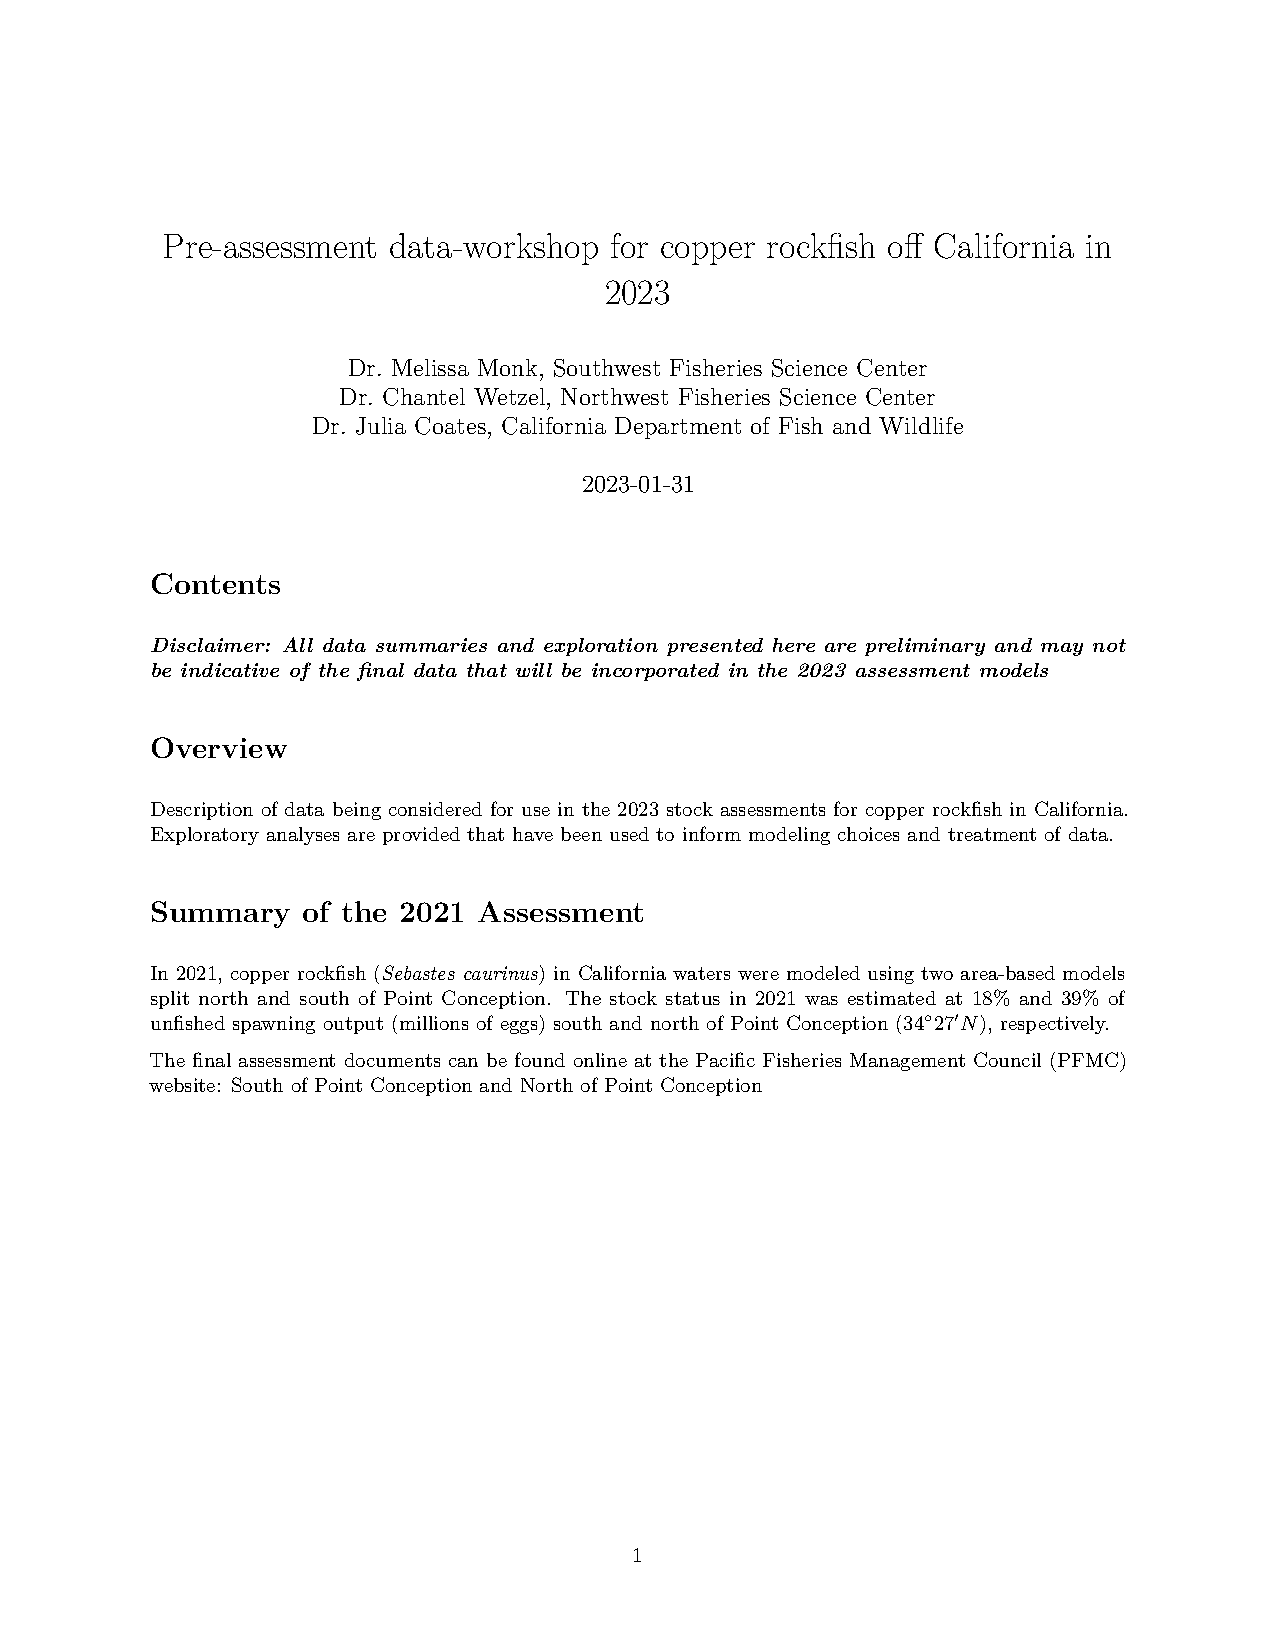
\includegraphics[width=1\textwidth,height=1\textheight]{S:/copper_rockfish_2023/data/rec_indices/crfs_pr_dockside/south/rm_last2yrs/index.png}
\caption{Index for the dockside PR survey.\label{fig:pr-index}}
\end{figure}

\newpage

\begin{figure}
\centering
\includegraphics[width=1\textwidth,height=1\textheight]{S:/copper_rockfish_2023/data/rec_indices/crfs_pr_dockside/south/rm_last2yrs/qq.png}
\caption{QQ plot for the dockside PR survey.\label{fig:pr-qq}}
\end{figure}

\newpage
\end{document}
